\documentclass[12pt]{article}

\usepackage[spanish]{babel}
\usepackage{hyperref}
\usepackage{graphicx}
\usepackage{listings}
\usepackage{color}
\usepackage{multicol}
\usepackage{amssymb}
\usepackage{enumitem}
\usepackage{here}
\usepackage{dsfont}
\usepackage{amsmath}
\usepackage{tipa}
\usepackage{float}
\spanishdecimal{.}

\title{Matemáticas para las Ciencias Aplicadas I}
\title{
	Tercera Lista de Problemas \\
	\textbf{Segunda  Parte} \\
	\vspace{1ex}
	\large Matemáticas para las Ciencias Aplicadas I \\
	Facultad de Ciencias, UNAM}

\date{\today}

\author{Flores Morán Julieta Melina \\ Zarco Romero José Antonio}

\begin{document}

\maketitle

%% De la sección 4.1: ejercicios 31, 57 y 71.
%% De la sección 4.2: ejercicios 31, 55 y 77.
%% De la sección 4.3: ejercicios 21, 36, 54 y 70.

%% 4.1 -----------------------------------------------------------------------------------------------------------------------------------------------------------------------------------------------------------------------------
\section{Sección 4.1 \\ Análisis De Funciones I: Aumento, Disminución Y Concavidad}
% 31 -------------------------------------------------------------------------------------------------------------
\subsection{Ejercicio 31} name \\

Encuentre: (a) los intervalos en los que $f$ aumenta, (b) los intervalos en los que $f$ disminuye, (c) los intervalos abiertos en los que $f$ es cóncava hacia arriba, (d) los intervalos abiertos en los que $f$ es cóncava hacia abajo, y (e) las coordenadas x de todos los puntos de inflexión.
\[
f(x) = \tan^{-1}(x^2-1)
\]

% 57 -------------------------------------------------------------------------------------------------------------
\subsection{Ejercicio 57} Zarco Romero José Antonio \\

\begin{enumerate}[label=(\alph*)]
\item Demuestre que un polinomio cúbico general
  \[
  f(x) = ax^3 + bx^2 + cx + d \qquad (a\neq 0)
  \]
  tiene exactamente un punto de inflexión.

  Calculando las dos primeras derivadas de $f$ obtenemos
  \begin{align*}
    f'(x)
    &= 3ax^2 + 2bx +c \\
    f''(x)
    &= 6ax +2b \\
    &= 6a\left(x+\frac{b}{3a}\right)
  \end{align*}
  Ahora, calculamos cuando ocurre $f''(x)=0$
  \begin{align*}
    6a\left(x+\frac{b}{3a}\right)
    &= 0\\
    x+\frac{b}{3a}
    &= 0 \\
    x
    &= -\frac{b}{3a}
  \end{align*}
  Así, conocemos entonces que $f$ cambia su dirección de concavidad en $x=-\frac{b}{3a}$. \\ 
  $\therefore -\frac{b}{3a}$ es el único un punto de inflexión.
  \
  \begin{flushright}
    $\blacksquare$
  \end{flushright}

\item Demuestre que si un polinomio cúbico tiene tres intersecciones en el eje $x$, entonces el punto de inflexión ocurre en el valor promedio de las intersecciones.

  Si $f(x)$ tiene 3 intersecciones con el eje $x$, entonces podemos expresarlo como
  \[
  f(x)=a(x-r_1​)(x-r_2​)(x-r_3​)
  \]
  donde $r_1,r_2$ y $r_3​$ son las raíces del polinomio.
  
  Si desarrollamos la ecuación anterior, también se puede expresar como
  \begin{align*}
    & a(x-r_1​)(x-r_2​)(x-r_3​) \\
    & = a(x^2-r_1x-r_2x+r_1r_2)(x-r_3) \\
    & = a(x^3-r_1x^2-r_2x^2+r_1r_2x-r_3x^2+r_1r_3x+r_2r_3x-r_1r_2r_3) \\
    & = a[x^3-(r_1+r_2+r_3)x^2+(r_1+r_2+r_3)x-r_1r_2r_3]
  \end{align*}

  Comparando términos con $ax^3 + bx^2 + cx + d$, se sigue que $b=-a(r_1+r_2+r_3)$. De este modo, al sustituir el valor de $b$ en el punto de inflexión $-\frac{b}{3a}$, tenemos que
  \[
  -\frac{b}{3a}= -\frac{-a(r_1+r_2+r_3)}{3a}=\frac{1}{3}(r_1+r_2+r_3)
  \]
  $\therefore $ El punto de inflexión ocurre en el valor promedio de las intersecciones
  \begin{flushright}
    $\blacksquare$
  \end{flushright}


\item Utilice el resultado del inciso (b) para encontrar el punto de inflexión del polinomio cúbico $f(x) = x^3-3x^2 + 2x$, y verifique su resultado usando $f''$ para determinar dónde $f$ es cóncava hacia arriba y cóncava hacia abajo.

  Primero, debemos reescribir $f(x)$
  \begin{align*}
    f(x)
    &= x^3-3x^2 + 2x\\
    &=x(x^2-3x+2)\\
    &=x(x-1)(x-2)
  \end{align*}
  donde las raíces del polinomio son $r_1=0,r_2=1$ y $r_3=2$. Sustituyendo estos valores en el resultado del insciso (b), tenemos que el punto de inflexión es igual a
  \begin{align*}
    \frac{1}{3}(r_1+r_2+r_3)
    &= \frac{1}{3}(0+1+2) \\
    &= \frac{1}{3}(3) \\
    &= 1
  \end{align*}
  Por lo que 1 es el punto de inflexión.

  Para verificar el resultado, calculamos las dos primeras derivadas de $f$ donde obtenemos que
  \begin{align*}
    f'(x)
    &= 3x^2 - 6x +2\\
    f''(x)
    &= 6x -6 \\
    &= 6 (x-1)
  \end{align*}
  Así, comprobamos que 1 es el punto de inflexión, pues es cuando $f''(x)=0$. Procedemos a tabular
  \begin{table}[H]
    \centering
    \begin{tabular}{c|c|c}
      \hline
      Intervalo & $f''(x) = 6(x-1)$ & Conclusión \\
      \hline
      $-\infty<x<1$ & - & $f$ es cóncava hacia abajo \\
      $1<x<-\infty$ & + & $f$ es cóncava hacia arriba \\
      \hline
    \end{tabular}
  \end{table}
  $\therefore $ El punto de inflexión es (1,0), $f$ es cóncava hacia arriba en el intervalo $(1,+\infty)$ y cóncava hacia abajo en el intervalo $(-\infty,1)$.
  
\end{enumerate}

% 71 -------------------------------------------------------------------------------------------------------------
\subsection{Ejercicio 71} name \\

Suponiendo que $A, k$ y $L$ son constantes positivas, verifique que la gráfica de $y=L/(1+Ae^{-kt})$ tiene un punto de inflexión en $\left( \frac{1}{k}\ln{A},\frac{1}{2}L \right)$.


%% 4.2 -----------------------------------------------------------------------------------------------------------------------------------------------------------------------------------------------------------------------------
\section{Sección 4.2 \\ Análisis De Funciones II: Extremos Relativos; Graficar Polinomios} 
% 31 -------------------------------------------------------------------------------------------------------------
\subsection{Ejercicio 31} Zarco Romero José Antonio \\

Utilice la derivada dada para encontrar todos los puntos críticos de $f$ y en cada punto crítico determine si ocurre un máximo relativo, un mínimo relativo o ninguno de los dos. Supongamos en cada caso que $f$ es continua en todas partes.
\[
f'(x)=\ln{\left( \frac{2}{1+x^2} \right)}
\]

Al establecer $1+x^2=0$ se obtiene que $x=\pm 1$, por tanto -1 y 1 son puntos críticos
  \begin{table}[H]
    \centering
    \begin{tabular}{c|c|c}
      \hline
      Intervalo & $f'(x) = \ln{\left( \frac{2}{1+x^2} \right)$ & Conclusión \\
      \hline
      $(-\infty,-1)$ & - & $f$ es decreciente \\
      $(-1,1)$ & + & $f$ es creciente\\
      $(1,+\infty)$ & - & $f$ es decreciente\\
      \hline
    \end{tabular}
  \end{table}
  Dado que el signo de $f'$ cambia de - a + en $x=-1$, hay uun mínimo relativo allí, y
  dado que el signo de $f'$ cambia de + a - en $x=1$, hay un máximo relativo allí.

  $\therefore $ Los puntos críticos son -1 y 1, en -1 ocurre un mínimo relativo y en 1 un máximo relativo.

% 55 -------------------------------------------------------------------------------------------------------------
\subsection{Ejercicio 55} name \\

Haz una gráfica del polinomio y etiqueta las coordenadas de las intersecciones, los puntos estacionarios y los puntos de inflexión. Comprueba tu trabajo con una utilidad gráfica.
\[
p(x) = (x + 1)^2 (2x-x^2 )
\]

% 77 -------------------------------------------------------------------------------------------------------------
\subsection{Ejercicio 77} Zarco Romero José Antonio \\

En cada parte, encuentre $k$ de modo que $f$ tenga un extremo relativo en el punto donde $x = 3$.
\begin{enumerate}[label=(\alph*)]
\item $f(x)=x^2+\frac{k}{x}$

  Calculando la primera derivada de $f$ obtenemos que
  \begin{align*}
    f'(x)
    &= 2x-\frac{k}{x^2} \\
    &= \frac{2x^3-k}{x^2}
  \end{align*}
  Cuando $f'(x)=0$, tenemos que
  \begin{align*}
    \frac{2x^3-k}{x^2}
    &=0\\
    2x^3-k
    &=0\\
    k
    &=2x^3\\
    k\vline_{x=3}
    &= 2(3)^3\\
    &=54
  \end{align*}
  $\therefore k=54$

\item $f(x)=\frac{x}{x^2+k}$
  

  Calculando la primera derivada de $f$ obtenemos que
  \begin{align*}
    f'(x)
    &= \frac{x^2+k-2x^2}{(x^2+k)^2}\\
    &= \frac{k-x^2}{(x^2+k)^2}
  \end{align*}
  Cuando $f'(x)=0$, tenemos que
  \begin{align*}
    \frac{k-x^2}{(x^2+k)^2}
    &=0\\
    k-x^2
    &=0\\
    k
    &=x^2\\
    k\vline_{x=3}
    &= (3)^2\\
    &=9
  \end{align*}
  $\therefore k=9$
\end{enumerate}

%% 4.3 -----------------------------------------------------------------------------------------------------------------------------------------------------------------------------------------------------------------------------
\section{Sección 4.3 \\  Análisis De Funciones III: Funciones Racionales, Cúspides Y Tangentes Verticales}
% 21 -------------------------------------------------------------------------------------------------------------
\subsection{Ejercicio 21} name \\

Dibuja una gráfica de la función racional y etiqueta las coordenadas de los puntos estacionarios y los puntos de inflexión. Muestra las asíntotas horizontales, verticales, oblicuas y curvilíneas y etiquétalas con sus ecuaciones. Etiquete los puntos, si los hay, donde la gráfica cruza una asíntota. Comprueba tu trabajo con una utilidad gráfica.
\[
\frac{(x-2)^3}{x^2}
\]

% 36 -------------------------------------------------------------------------------------------------------------
\subsection{Ejercicio 36} Zarco Romero José Antonio \\

Dé una gráfica de la función e identifique las ubicaciones de todos los puntos críticos y puntos de inflexión. Comprueba tu trabajo con una utilidad gráfica.
\[
5x^{2/3}+x^{5/3}
\]

Nos ayudará en nuestro análisis escribir
\[f(x)=5x^{2/3}+x^{5/3}=x^{2/3}(5+x)\]
\begin{itemize}
\item \textbf{Simetría}: No existen simetrías sobre los ejes de coordenadas ni sobre el origen.
\item \textbf{Intersecciones $x$ y $y$}: Al establecer $x^{2/3}(5+x)=0$ se obtienen las intersecciones $x=0,-5$. También, establecer $x=0$ produce la intersección con el eje $y$ en $y=0$.
\item  \textbf{Asíntotas verticales}: Ninguna, ya que $f(x) = 5x^{2/3}+x^{5/3}$ es continua en todas partes.
\item  \textbf{Comportamiento final}: 
  \begin{align*}
    \lim_{x \to +\infty}5x^{2/3}+x^{5/3} = \lim_{x \to +\infty} x^{2/3}(5+x) = +\infty \\
    \lim_{x \to -\infty} 5x^{2/3}+x^{5/3} = \lim_{x \to -\infty}  x^{2/3}(5+x) = -\infty 
  \end{align*}
\item \textbf{Derivadas}:
  \begin{align*}
    \frac{dy}{dx}
    &= f'(x) = \frac{10}{3}x^{-1/3} + \frac{5}{3}x^{2/3} = \frac{5}{3}x^{-1/3}(2+x)\\
    &= \frac{5(x+2)}{3x^{1/3}} 
  \end{align*}
  \begin{align*}
    \frac{d^2y}{dx^2}
    &= f''(x) = -\frac{10}{9}x^{-4/3} + \frac{10}{93}x^{-1/3} = \frac{10}{9}x^{-4/3}(-1+x) \\
    &= \frac{10(x-1)}{9x^{4/3}}
  \end{align*}
    \begin{table}[H]
    \centering
    \begin{tabular}{c|c|c}
      \hline
      Intervalo & $f''(x) = \frac{10(x-1)}{9x^{4/3}}$ & Conclusión \\
      \hline
      $(-\infty,0)$ & - & $f$ es cóncava hacia abajo \\
      $(0,1)$ & - & $f$ es cóncava hacia abajo \\
      $(1,+\infty)$ & + & $f$ es cóncava hacia arriba \\
      \hline
    \end{tabular}
  \end{table}
\item \textbf{Rectas tangentes verticales}: Hay una recta tangente vertical y cúspide en $x = 0$ ya que $f$ es continua allí y
  \begin{align*}
    \lim_{x \to 0^+} f'(x) = \lim_{x \to 0^+} \frac{5(x+2)}{3x^{1/3}}  = +\infty \\
    \lim_{x \to 0^-} f'(x) = \lim_{x \to 0^-} \frac{5(x+2)}{3x^{1/3}}  = -\infty 
  \end{align*}
\item \textbf{Conclusiones y gráfico}:
  \begin{itemize}
  \item Hay un punto crítico en $x = 0$ ya que $f$ no es diferenciable allí. Vimos arriba que en este punto se produce una cúspide.
  \item El análisis de signos de $f''(x)$ muestra que hay un punto de inflexión en $x = 1$, en el punto $(1,6)$, en el cual la gráfica cambia de cóncava hacia abajo a cóncava hacia arriba.
  \end{itemize}
\end{itemize}

Comparando con utilidad gráfica:
\begin{figure}[H]
\centering
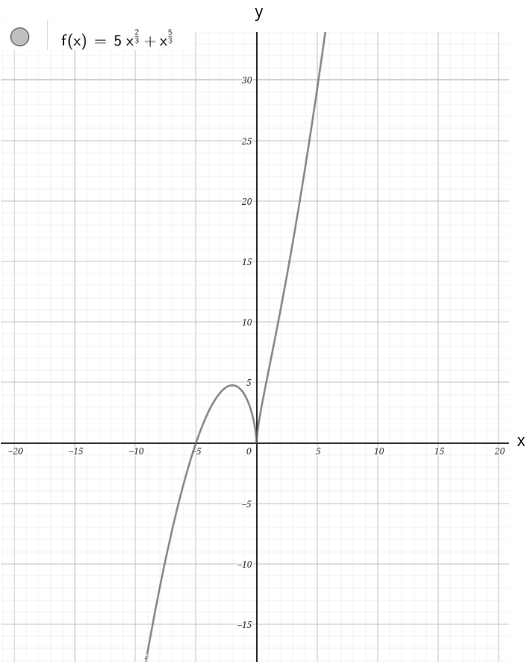
\includegraphics[width=0.8\textwidth]{../img/img_Lista3/p3_36.png}
\end{figure}



% 54 -------------------------------------------------------------------------------------------------------------
\subsection{Ejercicio 54} name \\

Utilizando la regla de L'Hôpital se puede verificar que
\begin{align*}
  \lim_{x \to +\infty} \frac{e^x}{x}=+\infty && \lim_{x \to +\infty} \frac{x}{e^x}=0 && \lim_{x \to -\infty} xe^x=0
\end{align*}
En estos ejercicios: (a) Utilice estos resultados, según sea necesario, para encontrar los límites de $f(x)$ cuando $x\rightarrow +\infty$ y cuando $x\rightarrow -\infty$. (b) Dibuje una gráfica de $f(x)$ e identifique todos los extremos relativos, puntos de inflexión y asíntotas (según corresponda). Comprueba tu trabajo con una utilidad gráfica.
\[
f(x)=x^3e^{x-1}
\]

% 70 -------------------------------------------------------------------------------------------------------------
\subsection{Ejercicio 70} name \\

La figura adjunta muestra una gráfica generada por computadora del polinomio $y = 0.1x^5 (x + 1)^2$ usando una ventana de visualización de $[−2, 1.5] \times [−0.2, 0.2]$. Demuestre que la elección de la escala vertical hizo que la computadora pasara por alto características importantes de la gráfica. Encuentra las características que faltaron y haz tu propio boceto del gráfico que muestra las características que faltan.
\begin{figure}[H]
\centering
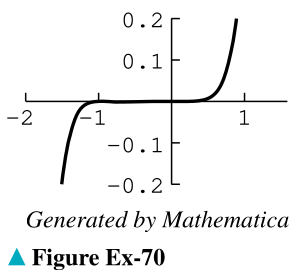
\includegraphics[width=0.4\textwidth]{../img/img_Lista3/2_70.png}
\end{figure}

\end{document}
